\documentclass{beamer}
\usepackage[utf8]{inputenc}
\usepackage{animate}
\usepackage{caption}
\usepackage{subcaption}
\definecolor{ntnublue}{RGB}{0, 80, 158}
\definecolor{burgundy}{RGB}{157, 0, 47}
\captionsetup{font={tiny, color = blue}, labelfont=tiny}
\usepackage{booktabs}
\usepackage{tabularx}
%\usetheme{Madrid}
\usetheme{Frankfurt}
%\usetheme{CambridgeUS}
%\usetheme{Berkeley}
%\usetheme{Hannover}
%\usetheme{Darmstadt}
%\usetheme{Warsaw}
%
\usecolortheme{beaver} 
%\usecolortheme{dolphin} 
%\usecolortheme{whale} 
%\usecolortheme{seahorse} 
%\usecolortheme{default}

\makeatletter
\setbeamertemplate{footline}{
  \leavevmode%
  \hbox{%
    \begin{beamercolorbox}[wd=.333\paperwidth,ht=2.5ex,dp=1.125ex,center]{author in head/foot}%
      \usebeamerfont{author in head/foot}\insertshortauthor
    \end{beamercolorbox}%
    \begin{beamercolorbox}[wd=.334\paperwidth,ht=2.5ex,dp=1.125ex,center]{title in head/foot}%
      \usebeamerfont{title in head/foot}\insertshorttitle
    \end{beamercolorbox}%
    \begin{beamercolorbox}[wd=.333\paperwidth,ht=2.5ex,dp=1.125ex,center]{date in head/foot}%
      \usebeamerfont{date in head/foot}\insertshortdate{}
      \hspace{2em}
      \insertframenumber{}/\inserttotalframenumber
    \end{beamercolorbox}%
  }%
  \vskip0pt%
}
\makeatother

\usepackage{tcolorbox}
\usepackage[backend = biber,
            style = apa,
            date = short,     % Long: 24th Mar. 1997 | Short: 24/03/1997
            sorting = nyt,
            url=false, 
            ]{biblatex} %customize the look of your citations and bibliography
% \usepackage[backend = biber,
%             style = ieee,
%             date = long,     % Long: 24th Mar. 1997 | Short: 24/03/1997
%             sorting = nyt,
%             maxcitenames = 1, 
%             maxbibnames = 99,
%             url=false, 
%             uniquename = false, 
%             uniquelist = minyear,
%             ]{biblatex} %customize the look of your citations and bibliography
\addbibresource{references_zotero.bib} %declare the bibliography resource
\let\cite\parencite


% USE this instead:
% \hypersetup{
%     colorlinks=true,
%     linkcolor=black,
%     citecolor=black,
%     urlcolor=blue
% }
%\usepackage{hyperref}   % load near the end of your preamble
\usepackage{xurl}       % AFTER hyperref — lets long urls/DOIs break anywhere

% Make biblatex print DOIs in a breakable way
\DeclareFieldFormat{doi}{%
  \mkbibacro{DOI}\addcolon\space
  \ifhyperref
    {\href{https://doi.org/#1}{\nolinkurl{#1}}}
    {\nolinkurl{#1}}}

\DeclareFieldFormat{url}{%
  \mkbibacro{URL}\addcolon\space
  \ifhyperref
    {\href{#1}{\nolinkurl{#1}}}
    {\nolinkurl{#1}}}




\addtobeamertemplate{footnote}{\vspace{-1ex}}{\vspace{12ex}}
\setbeamerfont{footnote}{size=\tiny}
%------------------------------------------------------------
%This block of code defines the information to appear in the
%Title page
\title[PhD Defence] %optional
{Contributions on acquisition and analysis of reflectance transformation imaging for cultural heritage applications}

%\subtitle{A short story}

\author[Khawaja] % (optional)
{Muhammad Arsalan Khawaja\inst{1,2}}

% {Muhammad Arsalan Khawaja\inst{1} \and J.~Doe\inst{2}}

\institute[NTNU-UBE] % (optional)
{
  \inst{1}%
  Colourlab, Department of Computer Science, \\
  Norwegian University of Science and Technology (NTNU),
  Gjøvik, Norway
  \and
  \inst{2}%
  ImViA Lab (UR7535),\\ Université Bourgogne Europe, Dijon, France
}

\date[18 June 2026] % (optional)
{\vspace{1cm} \color{ntnublue} PhD Thesis Defence}

\logo
{

\includegraphics[height=0.4cm]{figures/Logo_NTNU.png}
\hspace{0.5cm}

\includegraphics[height=0.54cm]{figures/Logo_Colourlab.png}
\hspace{0.5cm}

\includegraphics[height=0.6cm]{figures/Logo_ImVia.jpeg}
\hspace{0.5cm}

\includegraphics[height=0.45cm]{figures/Logo_spim.jpeg}
\hspace{0.5cm}

\includegraphics[height=0.87cm]{figures/Logo_UBE.png}
\hspace{0.05cm}
}


%End of title page configuration block
%------------------------------------------------------------



%------------------------------------------------------------
%The next block of commands puts the table of contents at the 
%beginning of each section and highlights the current section:

\AtBeginSection[]
{
  \begin{frame}
    
    \frametitle{Table of Contents}
    \tableofcontents[currentsection]
  \end{frame}
}
%------------------------------------------------------------


\begin{document}

%The next statement creates the title page.
{
\setbeamertemplate{headline}{}
\setbeamertemplate{footline}{}
\frame{\titlepage}
}



%---------------------------------------------------------
%This block of code is for the table of contents after
%the title page
{
\setbeamertemplate{headline}{}
\begin{frame}
\frametitle{Table of Contents}
\tableofcontents
\end{frame}
}
%---------------------------------------------------------


\section{Introduction}

\begin{frame}[t]
\frametitle{Imaging in Cultural Heritage (CH)}
    
    \begin{columns}

    \column{0.50\textwidth}

        \begin{itemize}
            \item<1-> Documentation.
            \item<2-> Digitization.
            \item<3-> Investigation.
        \end{itemize}

        \begin{block}<8->{\centering Reflectance Transformation Imaging (RTI)}
        \begin{itemize}
            \item<9-> Interactive virtual relighting.
            \item<10-> Captures directional appearance.
            \item<11-> 2.5D.
            \item<12-> Good resolution.
        \end{itemize}
        \end{block}

        % \begin{itemize}
        %     \item<8-> \color{ntnublue} Reflectance Transformation Imaging (RTI)
        %     \begin{itemize}
        %         \item 
        %     \end{itemize}
        % \end{itemize}

    \column{0.50\textwidth}

       \begin{itemize}
            \item<4-> Photography.
            \item<5-> 3D \& spatial imaging.
                \begin{itemize}
                    \item<2-> LiDAR \& laser scanning
                    \item<2-> Structured light scanning
                \end{itemize}
            \item<6-> Spectral imaging.
                \begin{itemize}
                    \item<6-> Hyperspectral imaging.
                    \item<6-> Infrared reflectography.
                \end{itemize}
            \item<7-> Microscopic imaging.
                \begin{itemize}
                    \item<7-> Optical microscopy.
                    \item<7-> Scanning electron microscopy.
                \end{itemize}
            \item<7-> Terahertz imaging, etc.
        \end{itemize}
        
    \end{columns}
    

\end{frame}



\begin{frame}
\frametitle{Reflectance Transformation Imaging (RTI)}

\begin{columns}

  \column{0.49\textwidth}

  \begin{itemize}
      \item<1-> What do you really need?
        \begin{itemize}
            \item<2-> Camera.
            \item<2-> Light source.
        \end{itemize}
      \item<3-> Optional
         \begin{itemize}
            \item<4-> Measuring tape.
            \item<4-> Reflective hemisphere.
        \end{itemize}     
      
  \end{itemize}


  \column{0.49\textwidth}
  
  \begin{figure}
    \centering
    \animategraphics[autoplay,loop,width=\columnwidth]{3}{figures/Animation_Acq/Def_RTI_acq_}{01}{07}
    \caption*{ Illustration of RTI acquisition. Coin source \footnotemark[1]}
  \end{figure}
\end{columns}

\footnotetext[1]{\tiny Coin: \url{https://sketchfab.com/3d-models/1-euro-coin-992424bd87714a29bcd4c58940e05ded} [Accessed: 04 April 2026].}

\end{frame}


\begin{frame}{Reflectance Transformation Imaging (RTI)}
  \centering
  \begin{minipage}[c][5.5cm][c]{\columnwidth}
    \centering
    \only<1>{
\includegraphics[width=\columnwidth, height=5.5cm, keepaspectratio]{figures/Animation_modeling/Def_Modeling_01.png}}%
    \only<2>{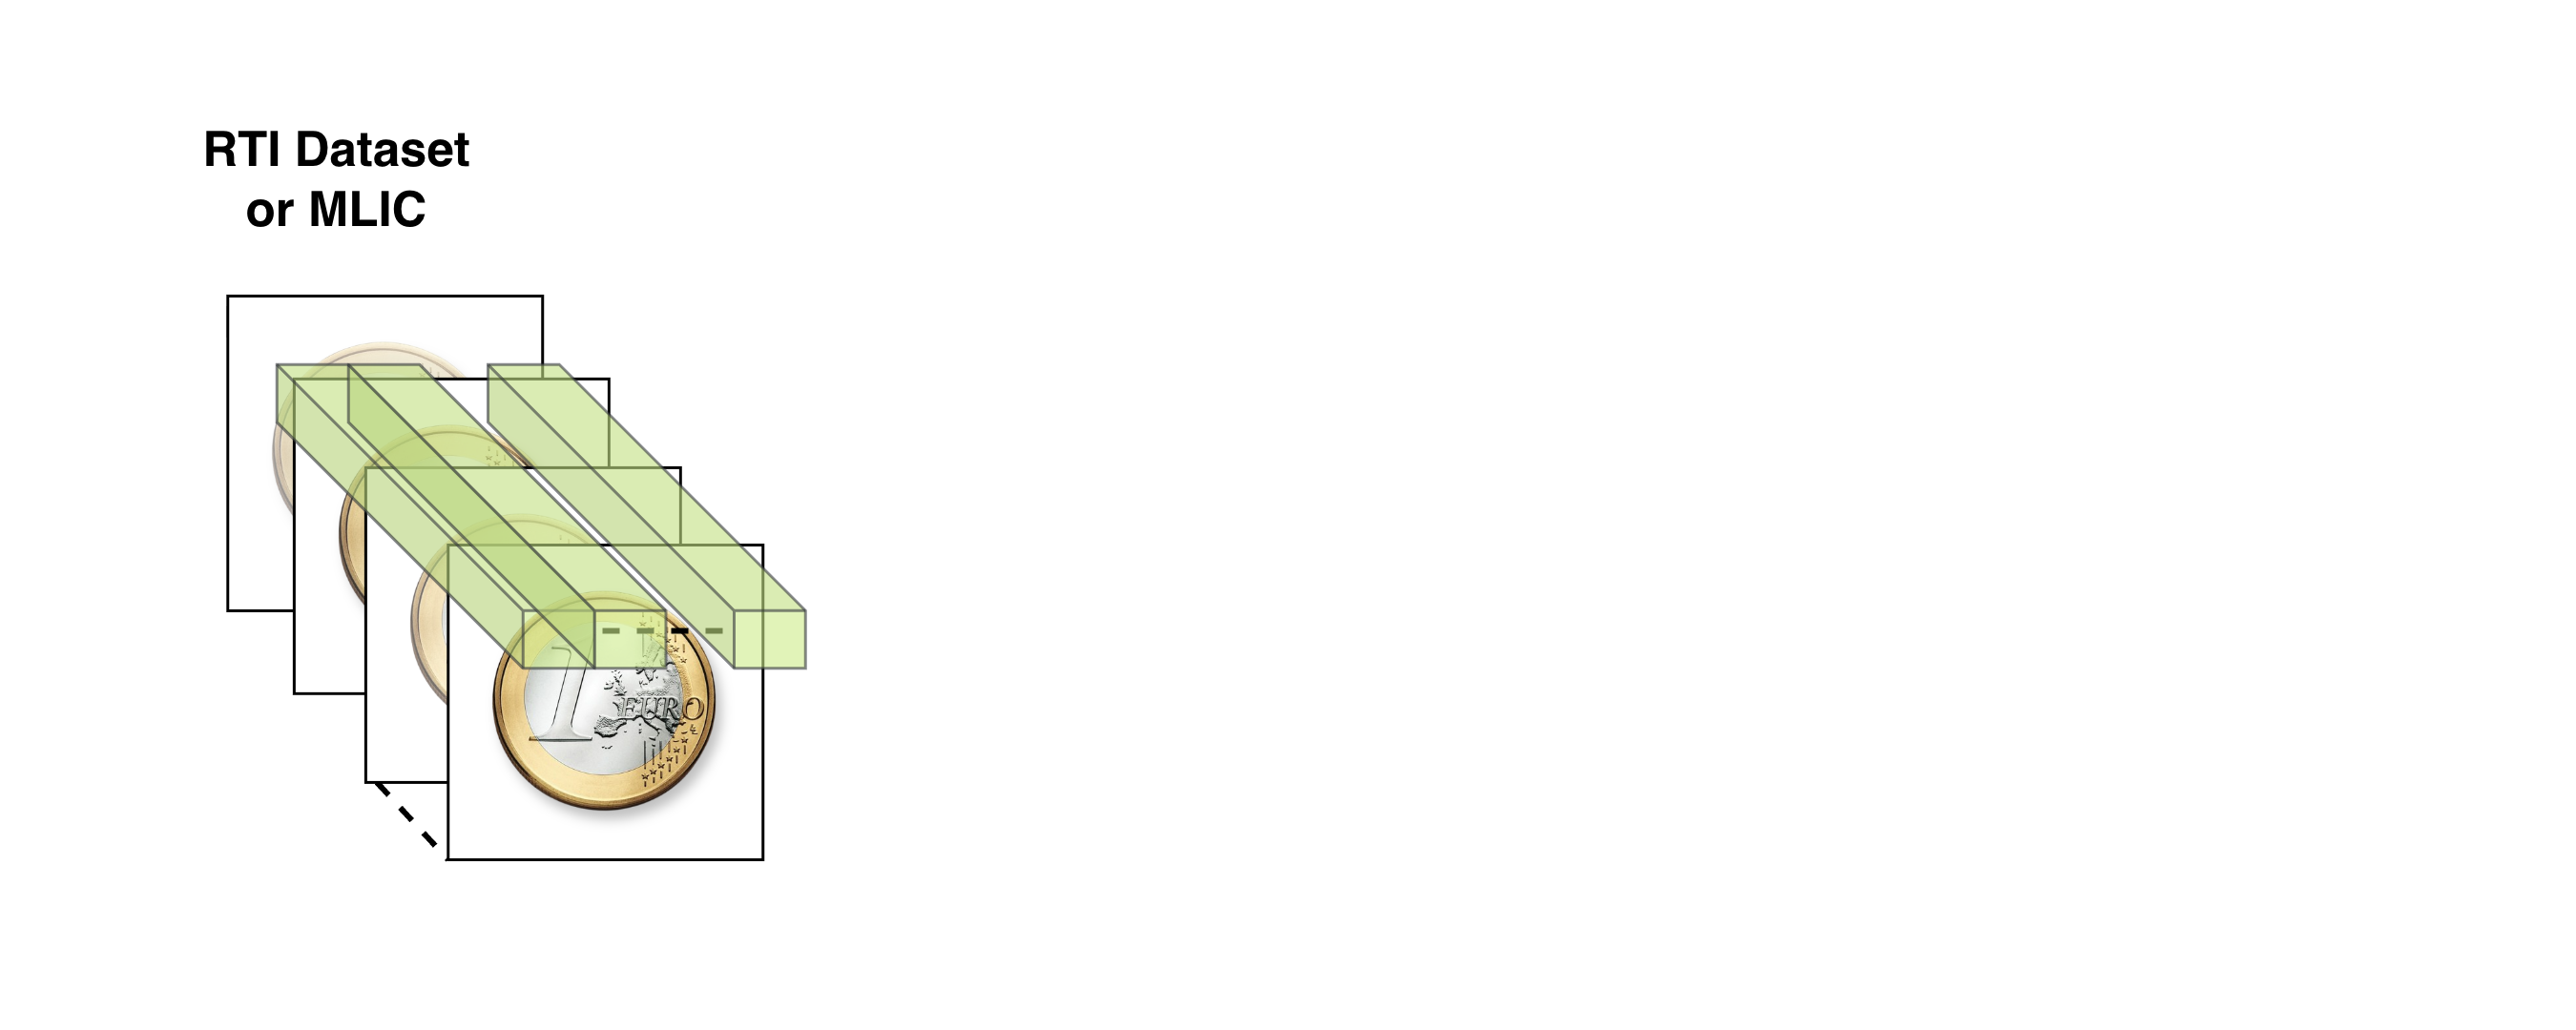
\includegraphics[width=\columnwidth, height=5.5cm, keepaspectratio]{figures/Animation_modeling/Def_Modeling_02.png}}%
    \only<3>{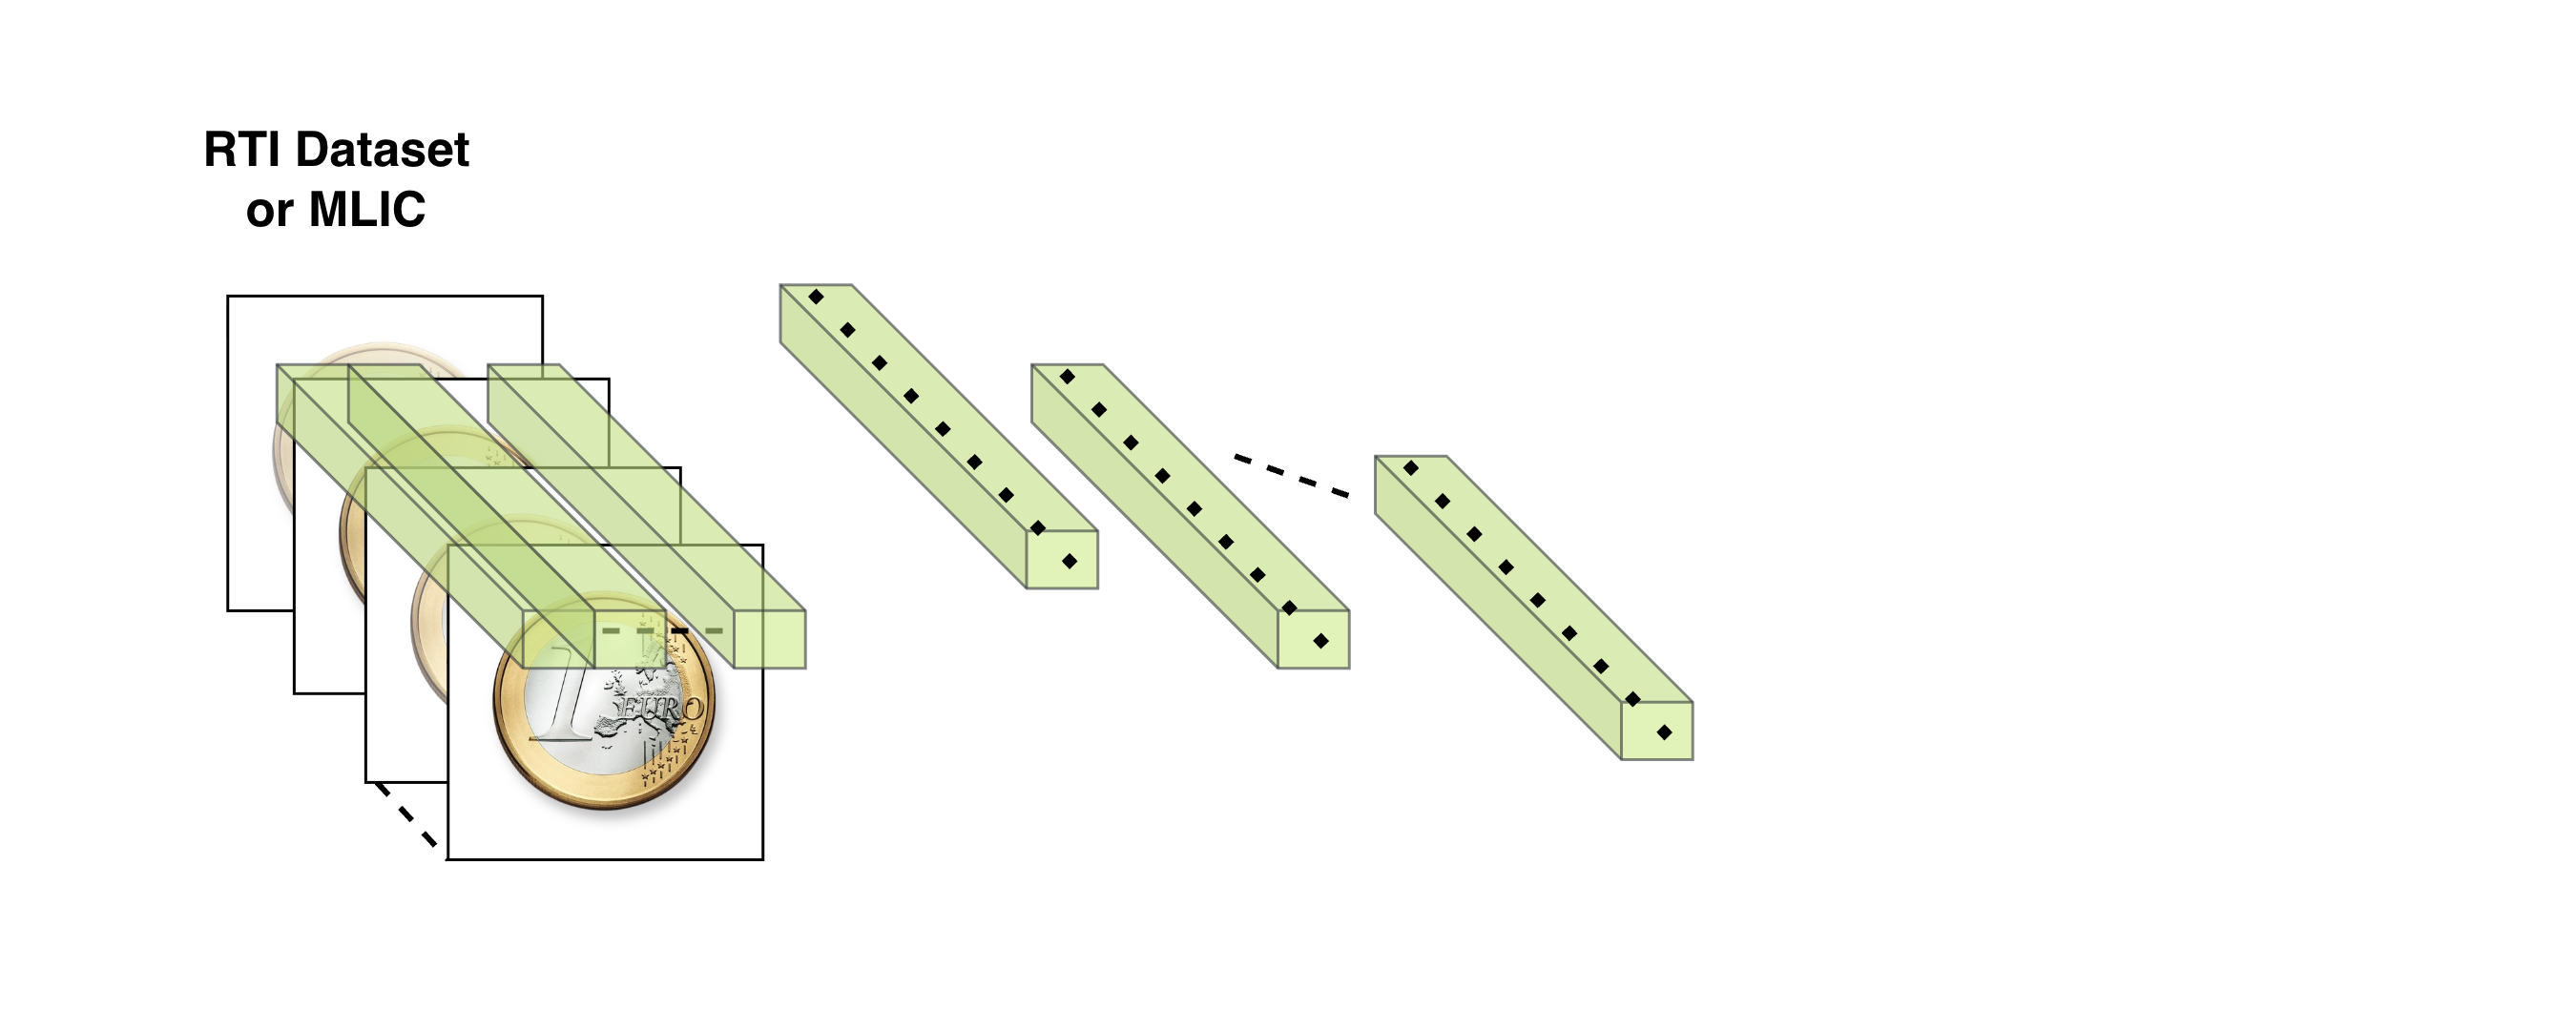
\includegraphics[width=\columnwidth, height=5.5cm, keepaspectratio]{figures/Animation_modeling/Def_Modeling_03.png}}%
    \only<4>{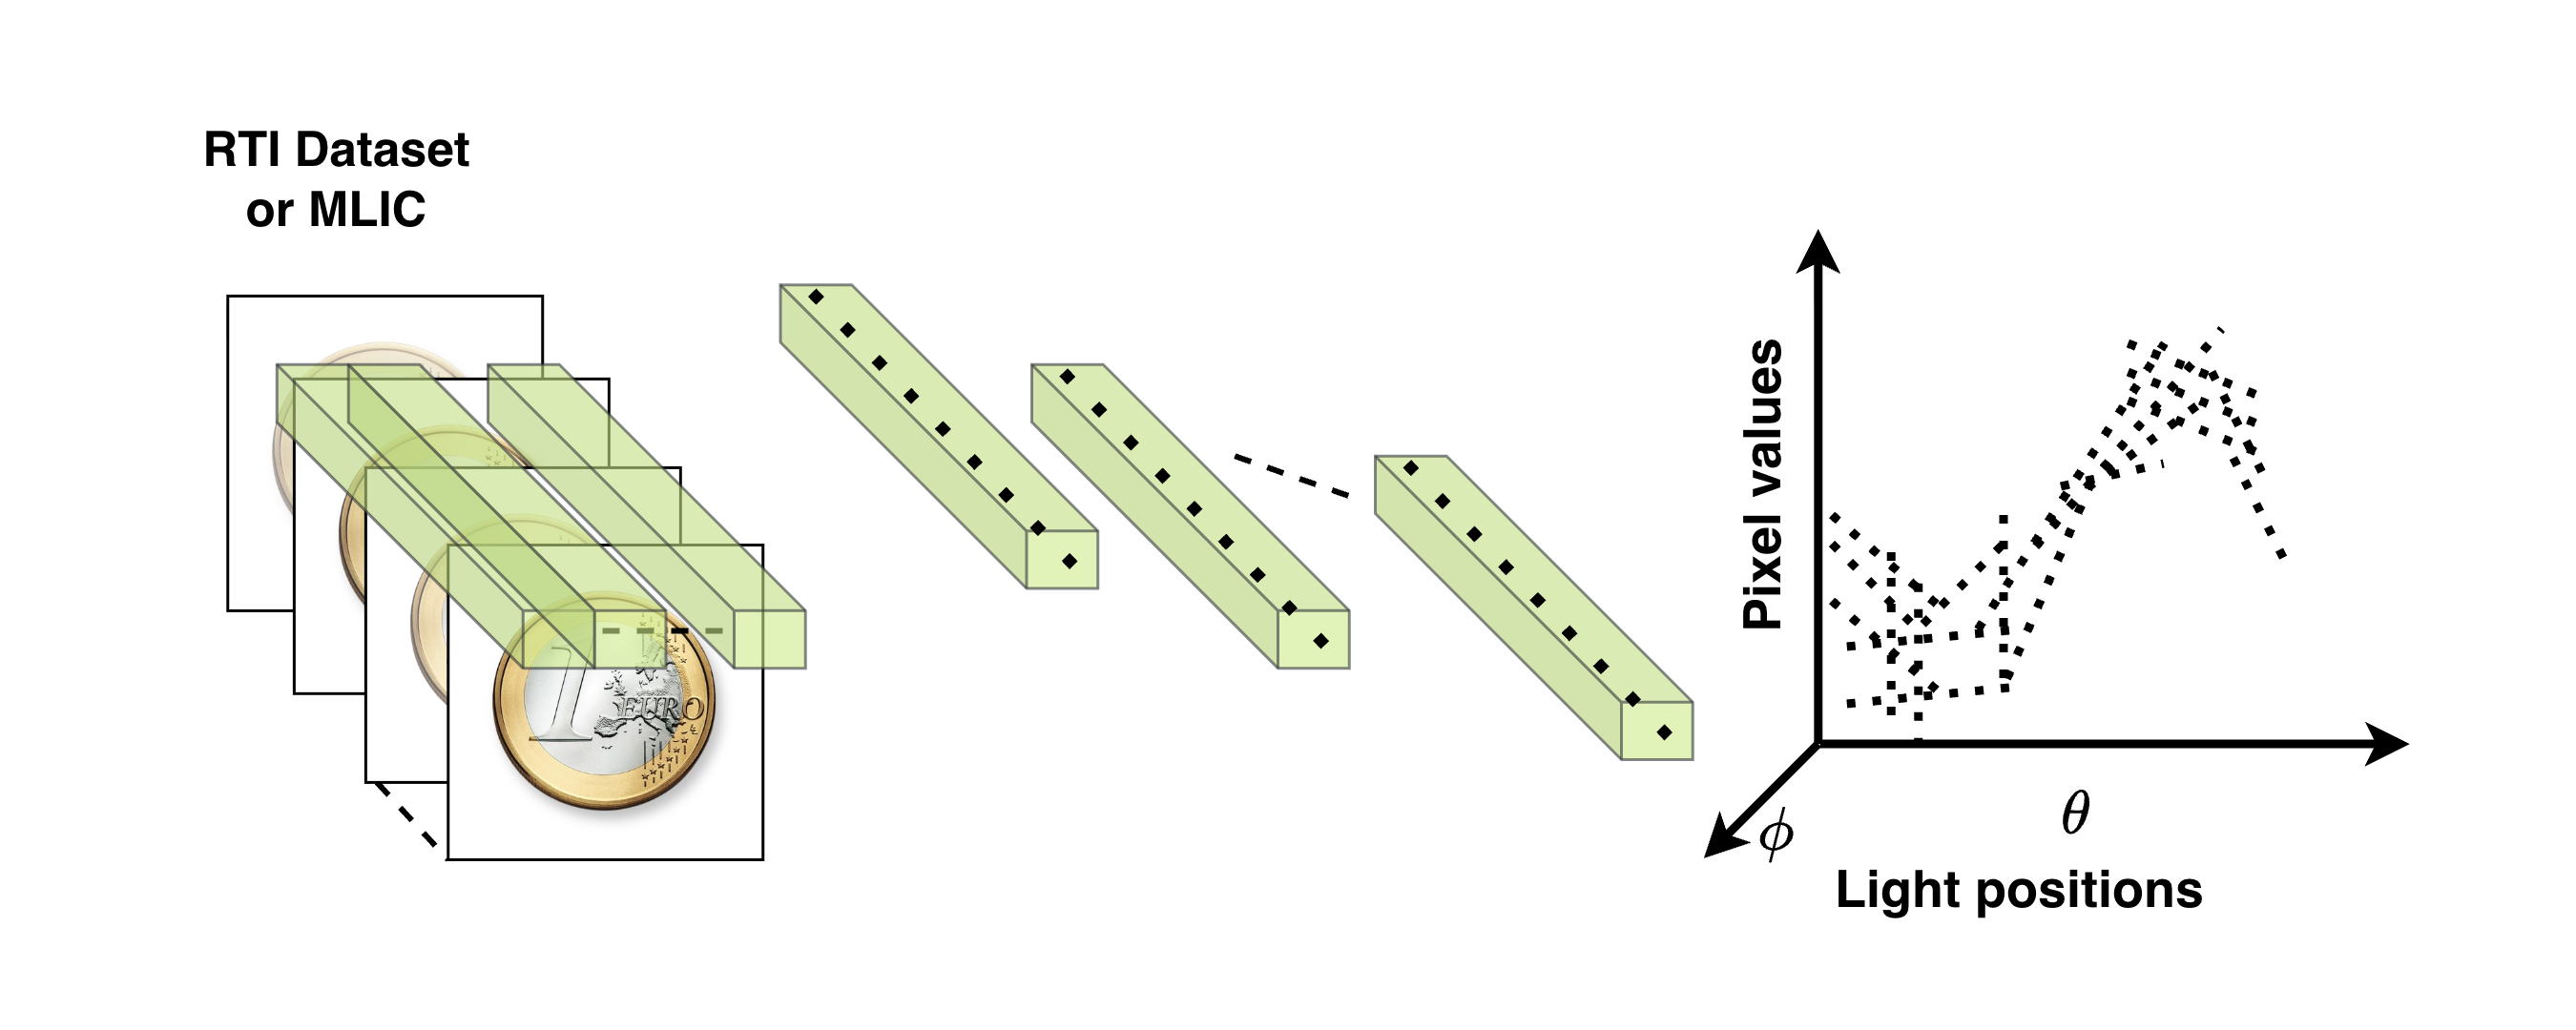
\includegraphics[width=\columnwidth, height=5.5cm, keepaspectratio]{figures/Animation_modeling/Def_Modeling_07.png}}%
    \only<5>{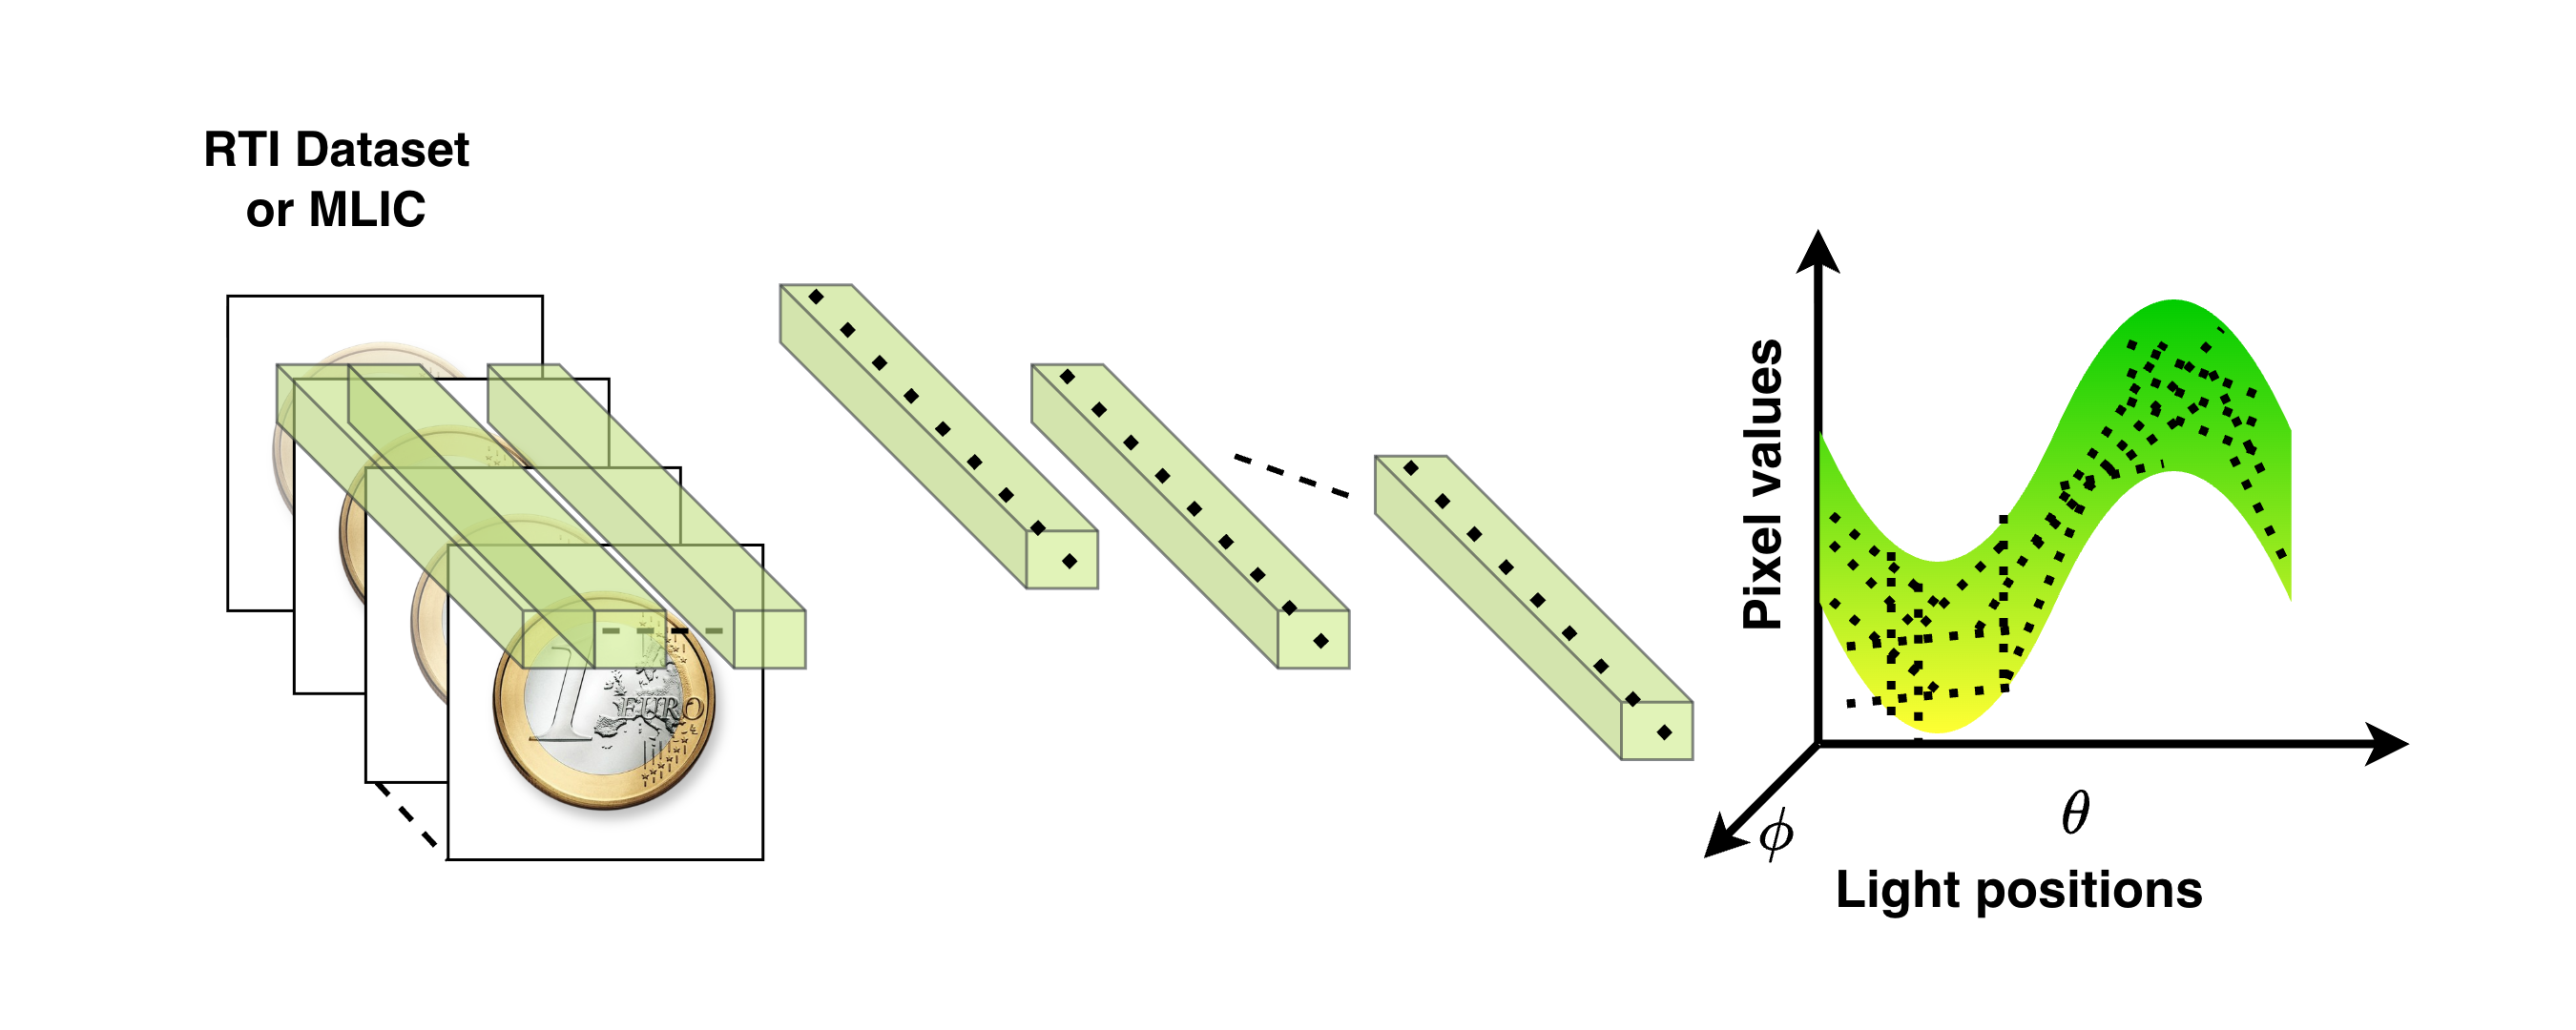
\includegraphics[width=\columnwidth, height=5.5cm, keepaspectratio]{figures/Animation_modeling/Def_Modeling_06.png}}%
    \only<6>{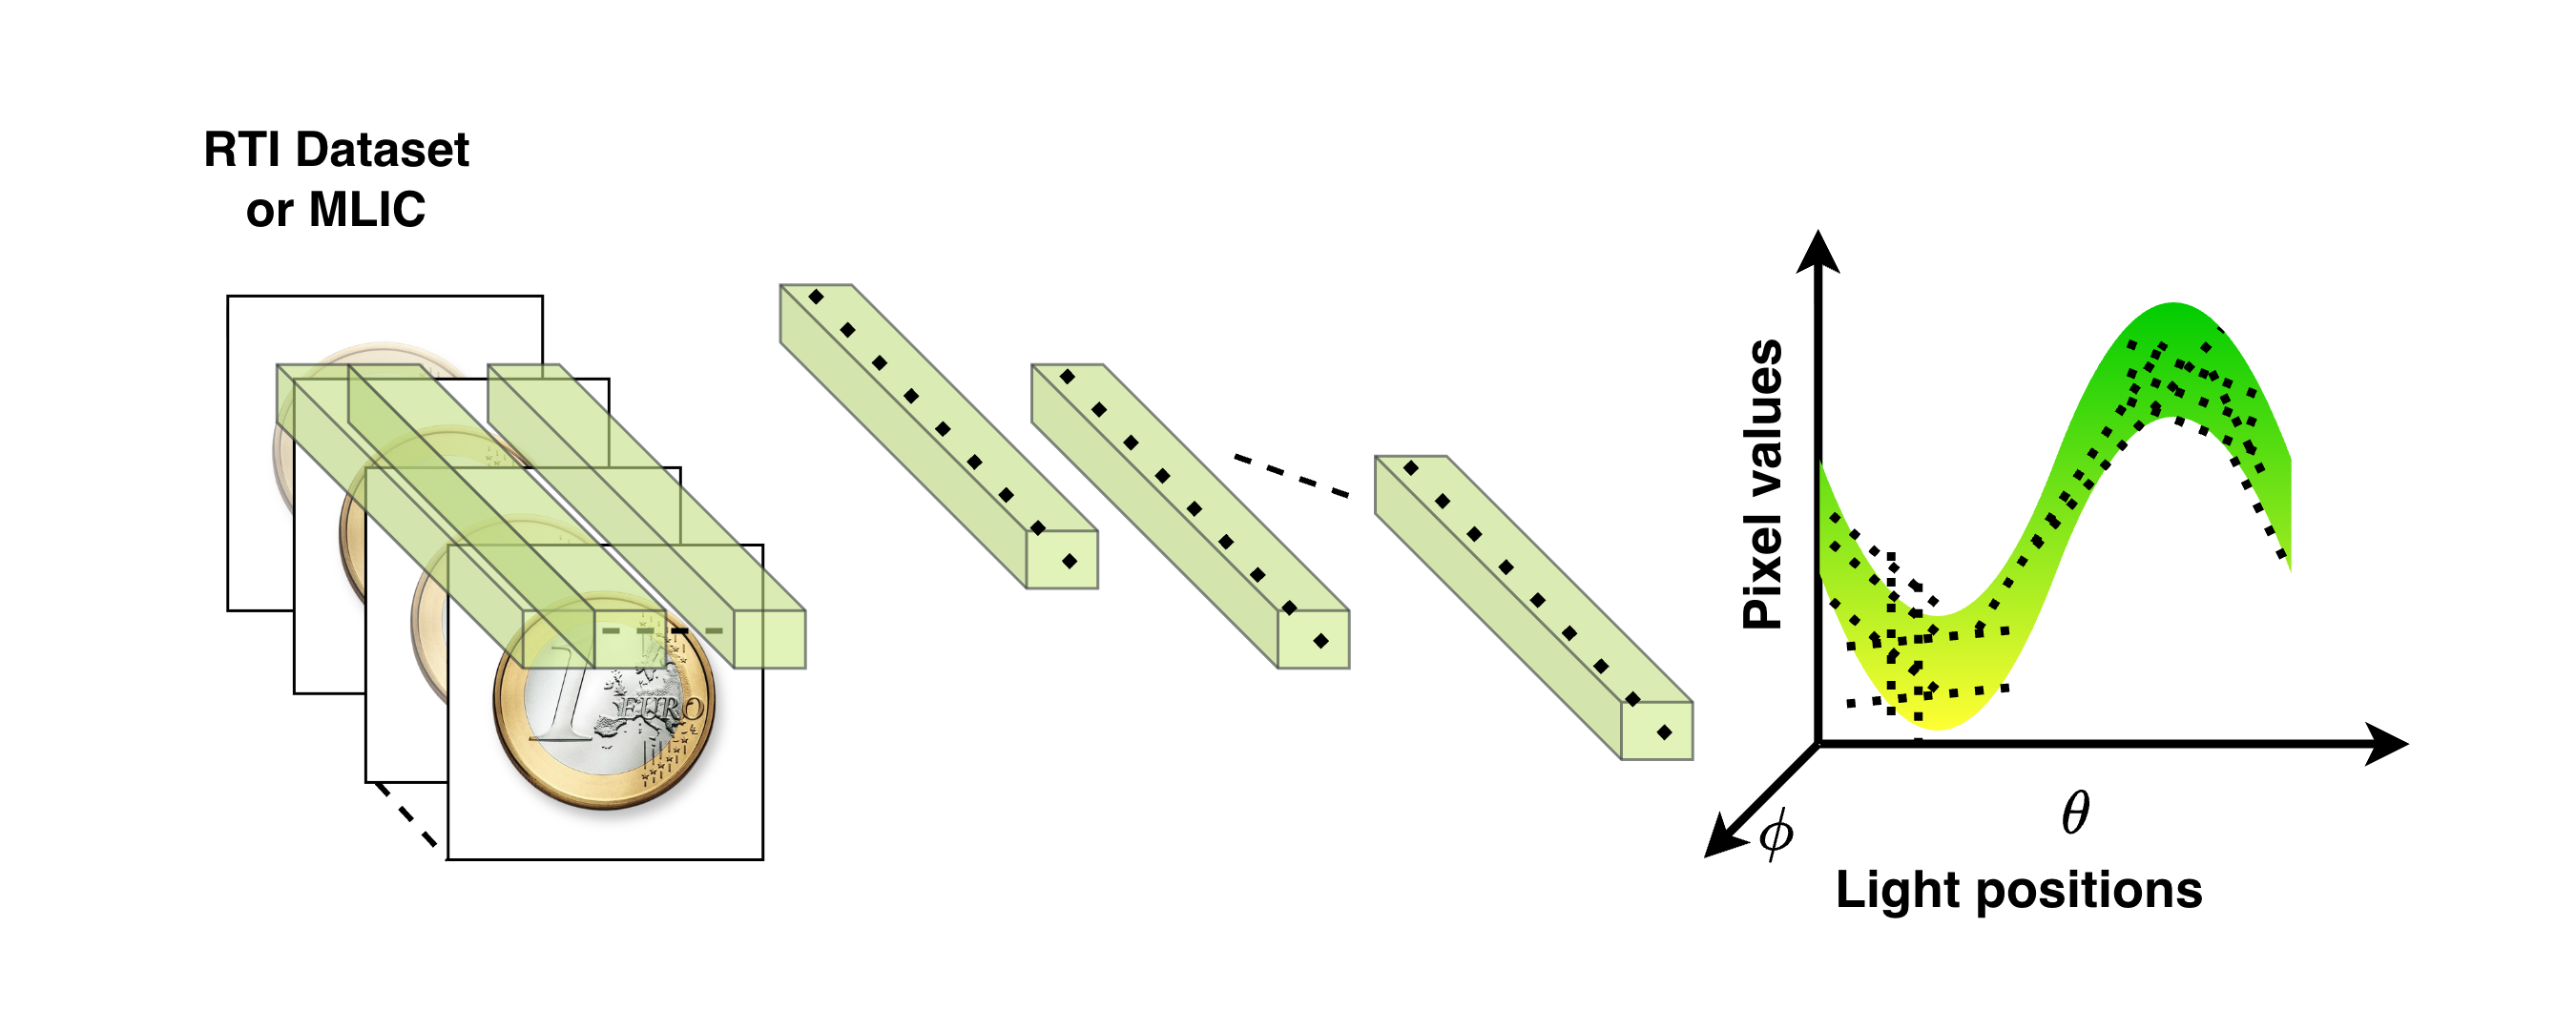
\includegraphics[width=\columnwidth, height=5.5cm, keepaspectratio]{figures/Animation_modeling/Def_Modeling_05.png}}%
    \only<7>{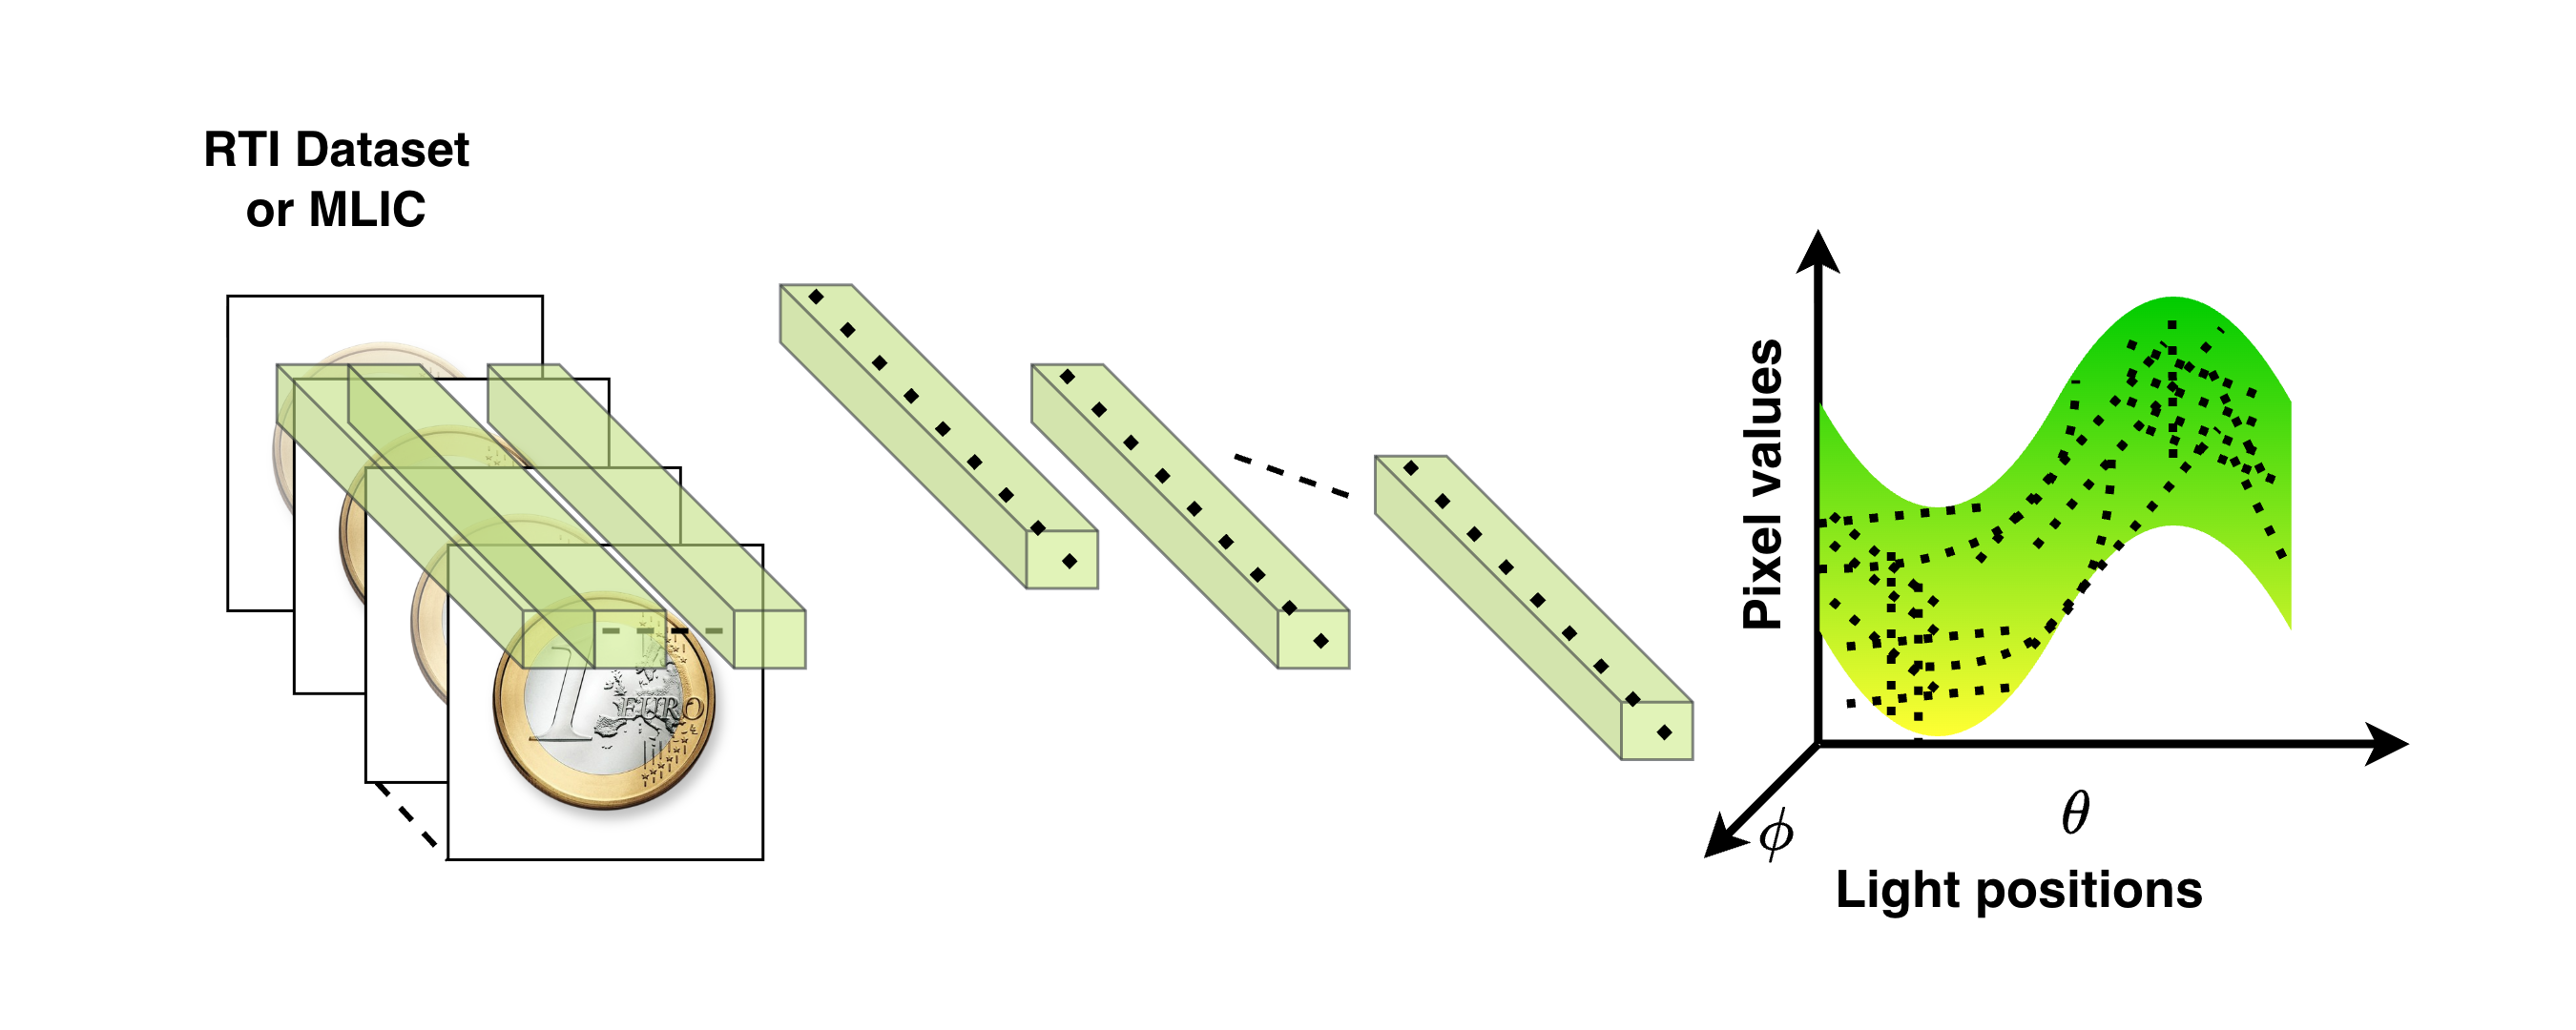
\includegraphics[width=\columnwidth, height=5.5cm, keepaspectratio]{figures/Animation_modeling/Def_Modeling_04.png}}%
  \end{minipage}
{\tiny\color{blue} Illustration of RTI modeling}  
\end{frame}


\begin{frame}{Reflectance Transformation Imaging (RTI)}
    
The final stage in RTI is application. These include:
    \begin{itemize}
        \item<1-> Interactive virtual relighting.
        \item<2-> Feature maps. 
        \item<3-> Normal map.
        \item<4-> Computational analysis.
    \end{itemize}
\end{frame}


\begin{frame}{Motivation}
    
\end{frame}

\begin{frame}{Research Questions}
    
\end{frame}

\begin{frame}{Research Papers}
\tiny
\renewcommand{\arraystretch}{1.3}
\resizebox{\textwidth}{!}{%
\begin{tabular}{>{\bfseries}p{1.2cm} p{7cm} p{3.5cm} p{1.8cm}}
\toprule
\textbf{Label} & \textbf{Title} & \textbf{Venue} & \textbf{Citation}\\
\midrule
Paper A & An interactive method for adaptive acquisition in RTI for cultural heritage.
  & ICCV Workshop, 2023, Paris & \cite{khawaja_interactive_2023} \\[4pt]
Paper B & Self-supervised classification of surfaces using RTI.
  & CVCS, 2024, Gjøvik & \cite{khawaja_self-supervised_2024} \\[4pt]
Paper C & RTI beyond relighting: Image analysis for archaeological Oseberg textiles.
  & London Imaging, 2025 & \cite{khawaja_rti_2025} \\[4pt]
Paper D & Beyond relighting: RTI deep learning for clustering heritage textiles.
  & npj Heritage Science & \cite{khawaja_beyond_2026} \\[4pt]
Paper E & Can Surface Topography Give Us Best Light Positions for RTI?
  & Archiving, 2023, Oslo & \cite{khawaja_can_2023} \\[4pt]
Paper F & Scene-adaptive RTI acquisition guided by dataset quality analysis.
  & Submitted to a journal& Preprint \\[4pt]
Paper G & SpheRTI: Spherical RTI for translucent surfaces.
  & Submitted to a journal& Preprint \\
\bottomrule
\end{tabular}%
}
\end{frame}


\begin{frame}[t]
\frametitle{Acquisition Setups}

\begin{columns}


  \column{0.5\textwidth}
  \begin{itemize}
    \item<1-> Free form RTI also known as Highlight RTI (H-RTI). 
        \begin{itemize}
            \item<1-> Lowest cost.
            \item<2-> Human or drone holds the light source.
        \end{itemize}
    \item<2-> Light positions can be estimated using reflective hemispheres.
  \end{itemize}

  \column{0.5\textwidth}
  \vspace{-0.5cm}
\begin{figure}[ht]
  \centering
  \begin{subfigure}{0.7\textwidth}
    \centering
    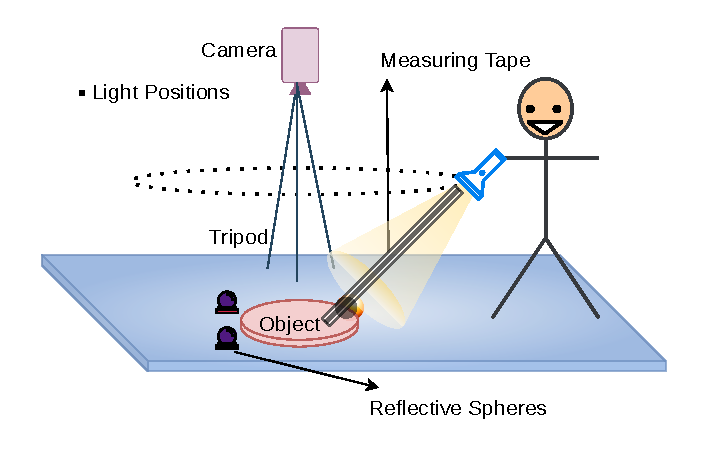
\includegraphics[width=\linewidth, trim={12 12 12 12}, clip]{figures/highligthRTI.pdf}
    \caption*{Human based (H-RTI)}
  \end{subfigure}
  
  \vspace{0.35cm}
  
  \begin{subfigure}{0.7\textwidth}
    \centering
    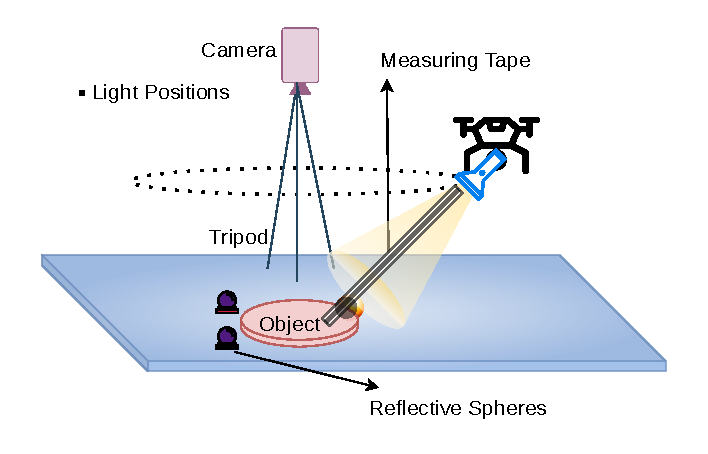
\includegraphics[width=\linewidth, trim={12 12 12 12}, clip]{figures/dronehighligthRTI.pdf}
    \caption*{Drone based (H-RTI)}
  \end{subfigure}  % optional overall caption
\end{figure}
  
\end{columns}
    
\end{frame}


%---------------------------------------------------------
\begin{frame}[t]
\frametitle{Acquisition Setups}

\begin{columns}


  \column{0.5\textwidth}
  \begin{itemize}
    \item<1-> Fixed multi-light setups.
        \begin{itemize}
            \item<1-> Quick acquisition. No flexible light positions.
            \item<2-> Lights are fixed in the dome structure.
        \end{itemize}
    \item<2-> No need for light position estimation using reflective hemispheres.
  \end{itemize}

  \column{0.5\textwidth}
  \vspace{-0.5cm}
\begin{figure}[ht]
  \centering
  \begin{subfigure}{0.7\textwidth}
    \centering
    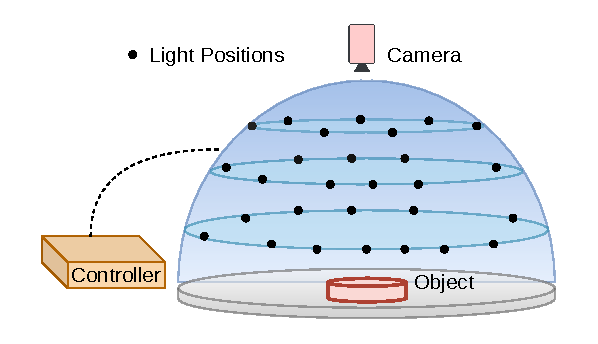
\includegraphics[width=\linewidth, trim={12 12 12 12}, clip]{figures/FixedlightDome.pdf}
    \caption*{Fixed light RTI with dome}
  \end{subfigure}
  
  \vspace{0.35cm}
  
  \begin{subfigure}{0.7\textwidth}
    \centering
    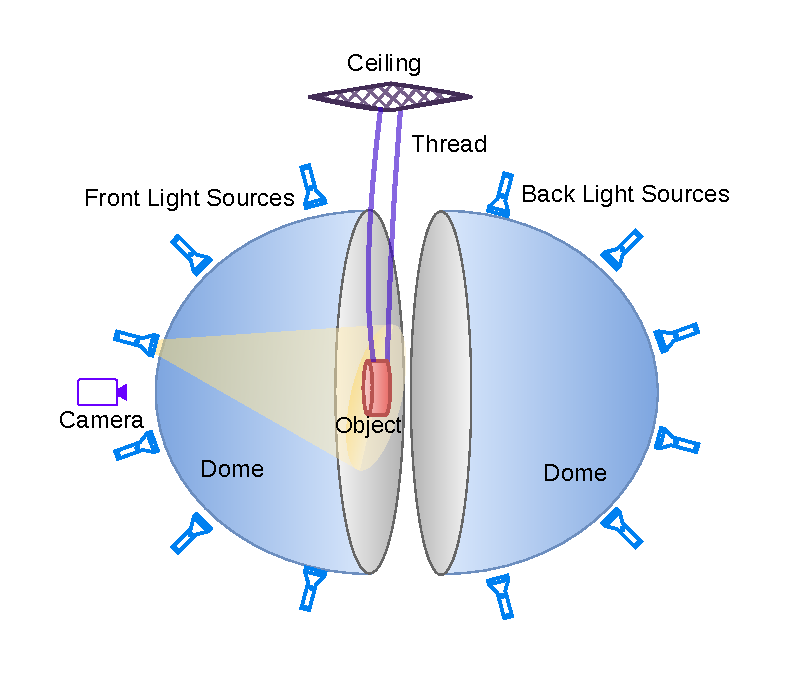
\includegraphics[width=\linewidth, trim={12 33 35 24}, clip]{figures/setupshpericalRTI.pdf}
    \caption*{Our proposed spherical RTI }
  \end{subfigure}  
\end{figure}
  
\end{columns}
    
\end{frame}


%---------------------------------------------------
\begin{frame}[t]
\frametitle{Acquisition Setups}

\begin{columns}


  \column{0.5\textwidth}
  \begin{itemize}
    \item<1-> Dynamic single-light setups.
        \begin{itemize}
            \item<1-> Relatively higher acquisition time. 
            \item<2-> Flexible light positions.
            \item<3-> Needs light planning, collision avoidance and robust to noise, etc.
        \end{itemize}
    \item<2-> No need for light position estimation using reflective hemispheres.
  \end{itemize}

  \column{0.5\textwidth}
  \vspace{-0.5cm}
\begin{figure}[ht]
  \centering
  \begin{subfigure}{0.6\textwidth}
    \centering
    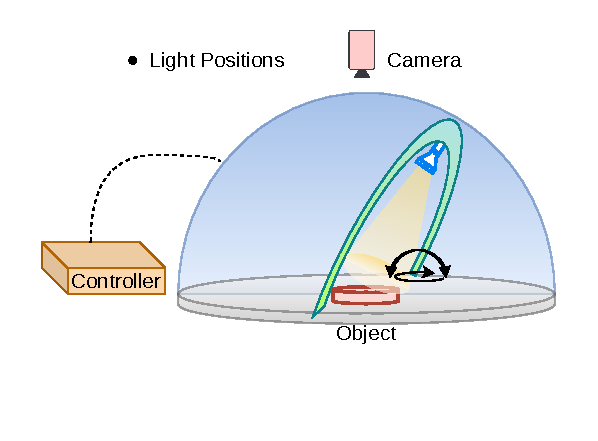
\includegraphics[width=\linewidth, trim={12 45 12 12}, clip]{figures/OnelightDome.pdf}
    \caption*{Fixed light RTI with dome}
  \end{subfigure}
  
  \vspace{0.7cm}
  
  \begin{subfigure}{0.6\textwidth}
    \centering
    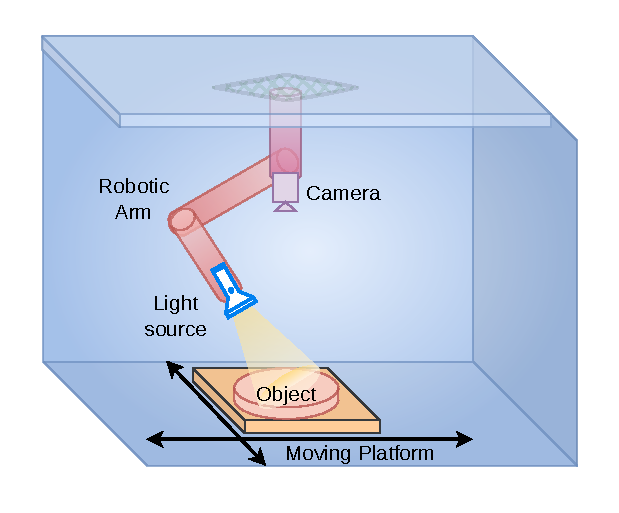
\includegraphics[width=\linewidth, trim={12 12 12 12}, clip]{figures/RoboticArmRTI.pdf}
    \caption*{Our proposed spherical RTI }
  \end{subfigure}  
\end{figure}
  
\end{columns}
    
\end{frame}


\begin{frame}{Modeling}
    
\end{frame}





%---------------------------------------------------------
%Changing visivility of the text
\begin{frame}
\frametitle{Introduction slide 1}
This is a text in second frame. For the sake of showing an example.

\begin{itemize}
    \item<1-> Text visible on slide 1
    \item<2-> Text visible on slide 2 \cite{khawaja_beyond_2026}
    \item<3> Text visible on slides 3
    \item<4-> Text visible on slide 4
    \item<5-> citing \cite{ansari-asl_advancing_2023}
\end{itemize}
\end{frame}

%---------------------------------------------------------


%---------------------------------------------------------
%Example of the \pause command
\begin{frame}
In this slide \pause

the text will be partially visible \pause

And finally everything will be there
\end{frame}


%---------------------------------------------------------
\section[Methods]{Methods}



% \subsection{Adaptive acquisition}


% \subsection{Surface Understanding}



%---------------------------------------------------------
\section[Results]{Results}



%---------------------------------------------------------

\section[Discussion]{Discussion}


%---------------------------------------------------------
\section[Conclusion]{Conclusion}



%---------------------------------------------------------


\begin{frame}{References}
  \renewcommand*{\bibfont}{\tiny}
  \printbibliography
\end{frame}



%---------------------------------------------------------




%---------------------------------------------------------



%---------------------------------------------------------
\section*{Appendix}

%---------------------------------------------------------
%Highlighting text
\begin{frame}
\frametitle{Sample frame title}

In this slide, some important text will be
\alert{highlighted} because it's important.
Please, don't abuse it.

\begin{block}{Remark}
Sample text
\end{block}

\begin{alertblock}{Important theorem}
Sample text in red box
\end{alertblock}

\begin{examples}
Sample text in green box. The title of the block is ``Examples".
\end{examples}
\end{frame}
%---------------------------------------------------------


%---------------------------------------------------------
%Two columns
\begin{frame}
\frametitle{Two-column slide}

\begin{columns}

\column{0.5\textwidth}
This is a text in first column.
$$E=mc^2$$
\begin{itemize}
\item First item
\item Second item
\end{itemize}

\column{0.5\textwidth}
This text will be in the second column
and on a second tought this is a nice looking
layout in some cases.
\end{columns}
\end{frame}
%---------------------------------------------------------


\end{document}